\subsubsection{Vision Data Analysis}

\begin{table}[h]
\caption{TextVQA dataset Rosetta OCR Error Analysis}
\label{ocr_error_analysis}
    \begin{center}
        \begin{tabularx}{\linewidth}{c|X X X}
            \hline
            \textbf{Dataset} & Error Rate & Detection Error Rate & Token Error Rate \\\hline
            \textbf{Training} & 29.17\% & 7.41\% & 23.50\% \\
            \textbf{Validation} & 40.55\% & 6.67\% & 31.58\% \\
            \textbf{Test} & 29.92\% & 15.35\% & 17.21\% \\
            \hline
            \textbf{Overall} & 32.05\% & 9.80\% & 24.67\% \\
            \hline
        \end{tabularx}
    \end{center}
\end{table}

We conduct exploratory analysis on vision data of TextVQA dataset, i.e., Rosetta OCR data following the original paper. To measure the error rate of OCR, we randomly sample 20 images from each of training set, validation set, and test set. \textit{Error Rate} measures the share of all incorrectly recognized tokens out of all detected boxes; \textit{Detection Error Rate} measures the share of OCR tokens generated from non-text boxes out of all detected boxes; and \textit{Token Error Rate} measures the recognition error rate among the detected boxes that do contain text, as shown in Table \ref{ocr_error_analysis}.

Moreover, the average numbers of objects and OCR tokens detected in each image are examined and presented in the Table \ref{obj_ocr_analysis}. It is worth noting that only 2897 out of 3289 images in the testing dataset are present in OpenImages' v0.6 dataset, which should contain all the image data according to the TextVQA web page.


\begin{table}[h]
\caption{Exploratory Analysis on Object \& OCR Tokens Detection }
\label{obj_ocr_analysis}
    \begin{center}
        \begin{tabularx}{\linewidth}{c|X X}
            \hline
            \textbf{Dataset} & Avg objects detected & Avg OCR tokens \\\hline
            \textbf{Training} & 5.04 & 12.45 \\
            \textbf{Validation} & 5.31 & 12.89 \\
            \textbf{Test} & 9.14$^1$ & 9.60 \\
            \hline
        \end{tabularx}
    \end{center}
    \begin{tablenotes}
        \item $^1$ Only 2897 out of 3289 testing images are present in OpenImages' v0.6 dataset
  \end{tablenotes}
\end{table}

By glancing over the data with OCR visualization, we conclude several troublesome problems of the Rosetta OCR data:
  \begin{enumerate}
    \item OCR tokens are designed to provide the model with answer candidates. A high \textit{Detection Error Rate} provides the model with more confusing and meaningless answer candidates; a high \textit{Token Error Rate}, even when the model can "copy" the correct answer space, brings the final accuracy down due to the incorrect recognition.
    \item Rosetta OCR recognizes each detection box into one token, which possibly consists of several words. The combination of the word, even each recognized correctly, is useless for the question answering model.
  \end{enumerate}
 
We present several typical errors in the model answering related to OCR data in Figure \ref{fig:ocr}. Specifically, Fig \ref{fig:incorrect_recognition} shows an image where correct answer can be "copied" from the OCR token, however, the OCR token is recognized incorrectly; Fig \ref{fig:multi_tokens_needed} detects and recognizes correctly, but multi tokens should be combined together as the answer; Fig \ref{fig:not_detected} has an answer that can be "copied" from the OCR token as well, whereas the answer is not detected by OCR model; Fig \ref{fig:partially_covered} is not answered correctly because the answer token is partially covered and OCR model is not able to complete it; Fig \ref{fig:ocr_not_helpful} has partial answer token correctly detected and recognized, however, the OCR is not helpful to obtain the rest part of the answer.

\begin{figure*}
\centering

\begin{subfigure}[b]{.4\textwidth}
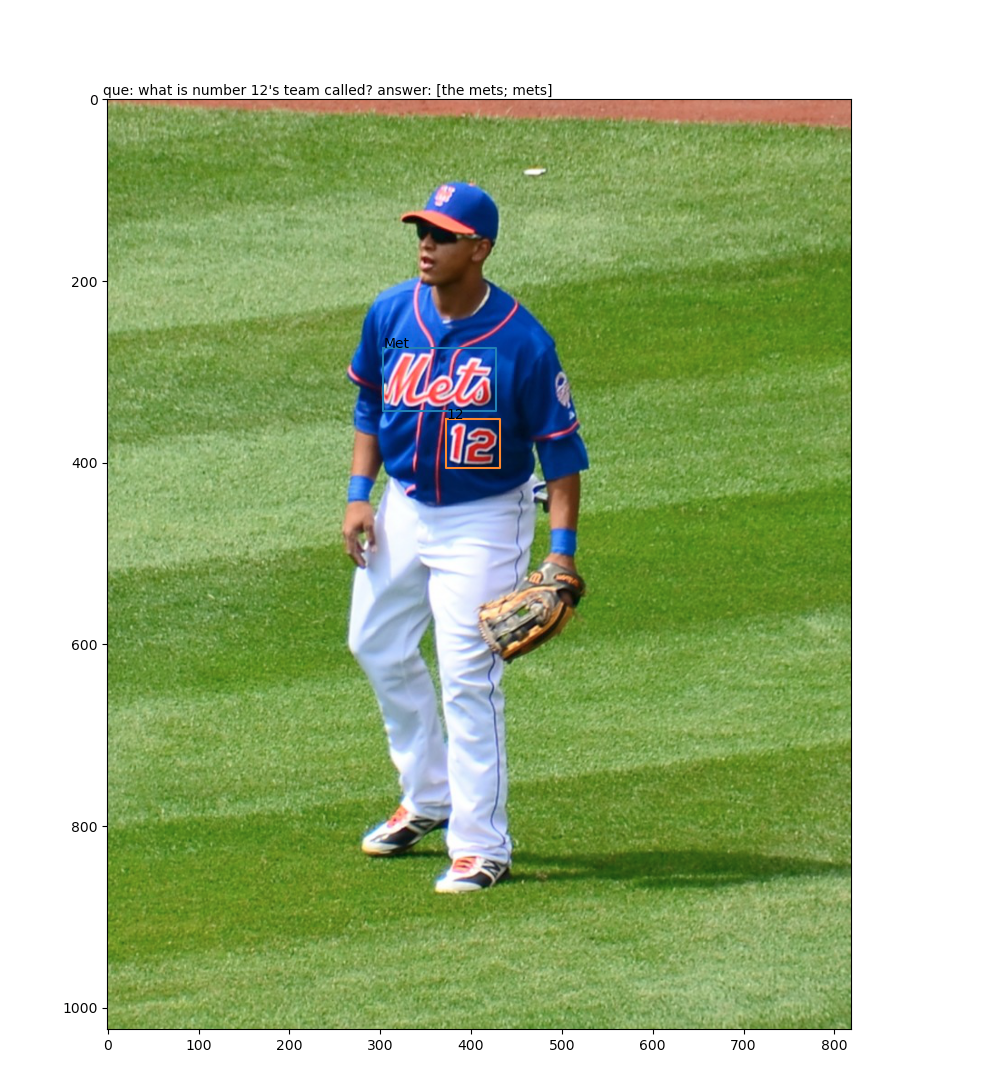
\includegraphics[width=\linewidth]{figures/incorrect_recognition.png}
\caption{Incorrect Recognition}\label{fig:incorrect_recognition}
\end{subfigure}
\begin{subfigure}[b]{.4\textwidth}
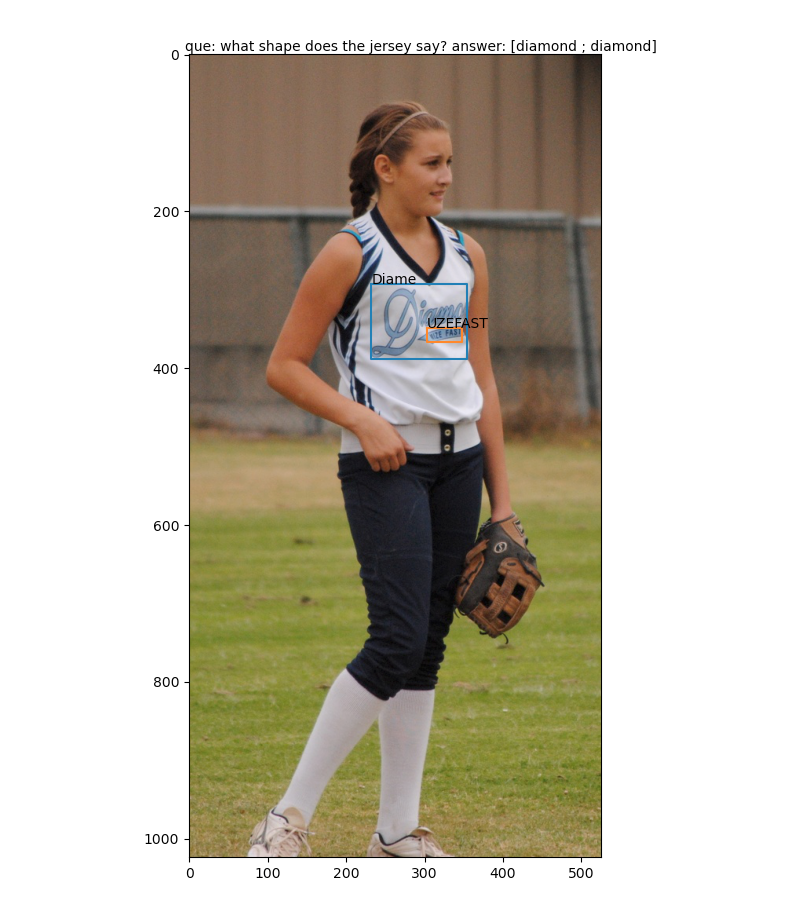
\includegraphics[width=\textwidth]{figures/partially_covered.png}
\caption{Text Partially Covered}\label{fig:partially_covered}
\end{subfigure}
\begin{subfigure}[b]{.33\textwidth}
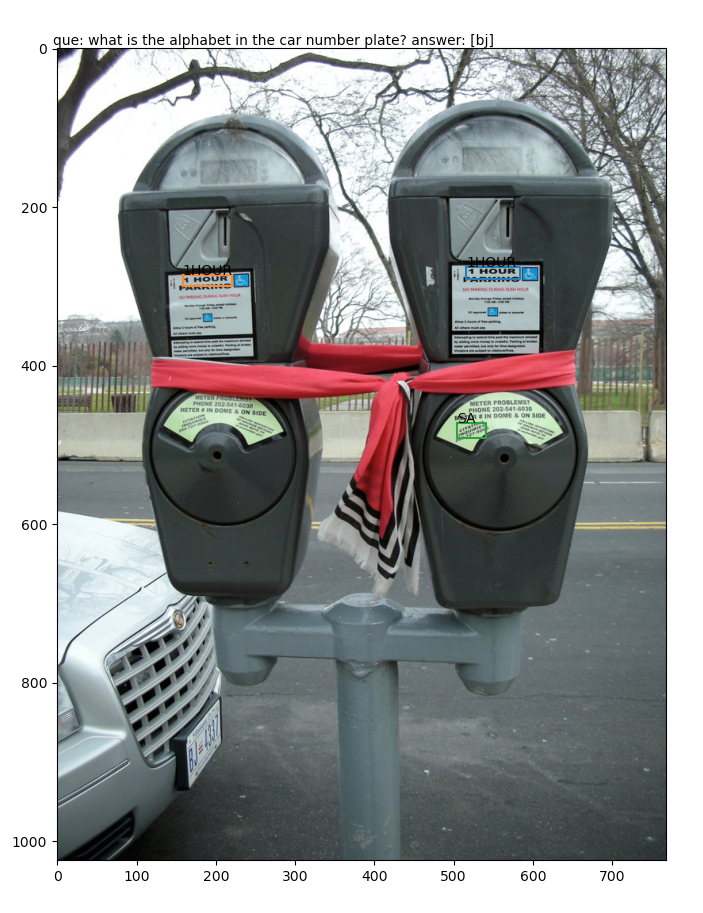
\includegraphics[width=\textwidth]{figures/not_detected.png}
\caption{Answer Not Detected}\label{fig:not_detected}
\end{subfigure}
\begin{subfigure}[b]{.5\textwidth}
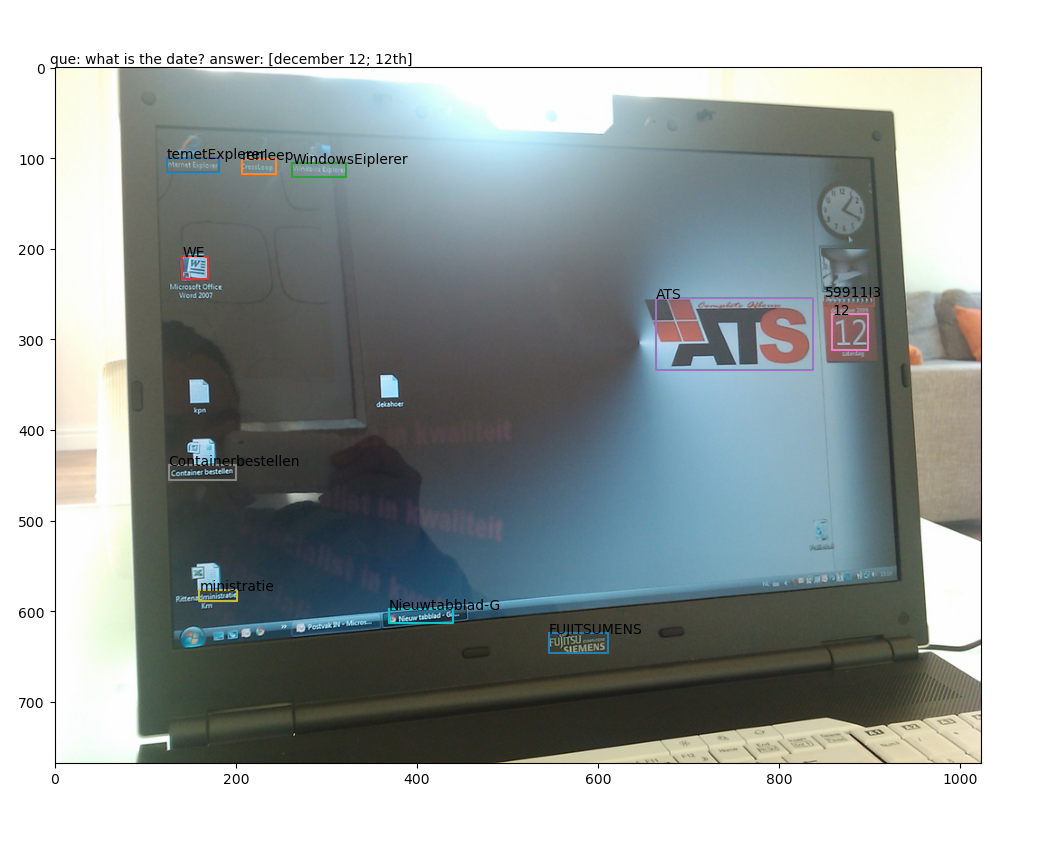
\includegraphics[width=\textwidth]{figures/ocr_not_helpful.png}
\caption{OCR Not Helpful}\label{fig:ocr_not_helpful}
\end{subfigure}
\begin{subfigure}[b]{.5\textwidth}
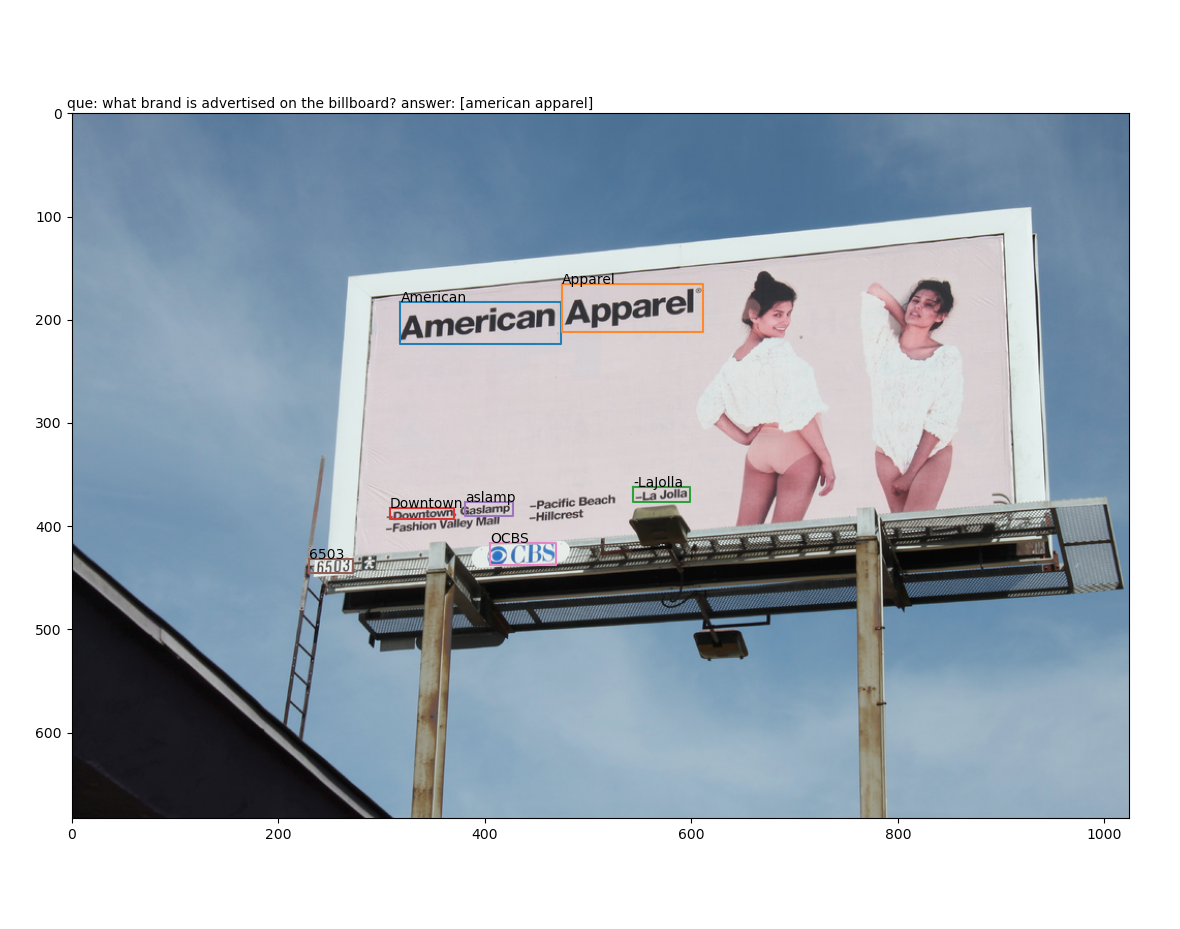
\includegraphics[width=\textwidth]{figures/multi_tokens_needed.png}
\caption{Need Multi Tokens}\label{fig:multi_tokens_needed}
\end{subfigure}

\caption{Typical errors related to OCR data.}
\label{fig:ocr}
\end{figure*}
